\documentclass[12pt]{article}
\usepackage{hhline}
\usepackage{graphicx}
\graphicspath{{pictures/}}
\DeclareGraphicsExtensions{.png}
\usepackage{multirow}
\usepackage{amsmath}
\usepackage{mathtext}
\usepackage[T2A]{fontenc}
\usepackage[utf8]{inputenc}
\usepackage{pscyr} 
\usepackage[ left=2cm,right=2cm, top=1.5cm,bottom=1cm,bindingoffset=0cm]{geometry}

\begin{document}
\pagestyle{empty}
\begin{center}
\large{\textbf{Университет ИТМО}}
\end{center}
\rule{500pt}{1pt}
\par\bigskip\par\bigskip\par\bigskip\par\bigskip\par\bigskip\par\bigskip\par\bigskip\par\bigskip
\begin{center}
\Large
\textbf{Отчёт по лабораторной работе №5}

\textbf{\textit{«Определение изобарной, изохорной теплоемкостей и коэффициента Пуассона воздуха в процессе адиабатного сжатия»}}


\end{center}
\par\bigskip\par\bigskip\par\bigskip\par\bigskip\par\bigskip\par\bigskip\par\bigskip\par\bigskip\par\bigskip\par\bigskip\par\bigskip\par\bigskip\par\bigskip\par\bigskip      
\begin{flushright}
\large
Выполнил: Федюкович С. А.
\par\bigskip
Факультет: МТУ “Академия ЛИМТУ”
\par\bigskip
Группа: S3100                       
\par\bigskip\par\bigskip\par\bigskip

\rule{150pt}{0.5pt}
\par\bigskip\par\bigskip\par\bigskip\par\bigskip                                                            
 Проверил: Пшеничников В. Е. 
\par\bigskip \par\bigskip

\rule{150pt}{0.5pt}
\end{flushright}
\par\bigskip\par\bigskip\par\bigskip\par\bigskip\par\bigskip\par\bigskip\par\bigskip\par\bigskip\par\bigskip\par\bigskip     
\begin{center}
\large
Санкт-Петербург
\par\bigskip
2018
\end{center}
\newpage

\section*{Цель работы}
По результатам комбинированного термодинамического процесса, проведенного над газом (воздухом), рассчитать значения изобарной, изохорной теплоемкостей, а также коэффициента Пуассона.
\section*{Теоретические основы лабораторной работы}
В данной работе над газом проводится комбинированный термодинамический процесс, состоящий из последовательно протекающих адиабатного и изохорного процессов. Диаграмма процессов:
\begin{center}
 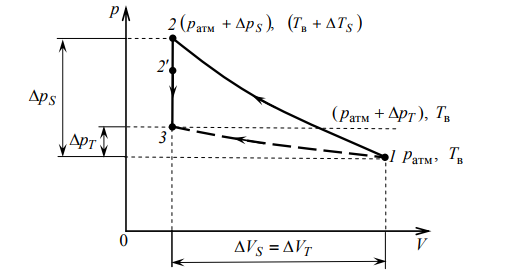
\includegraphics{1}
 \end{center} 
Вначале газ с параметрами $p_{атм}$ и  $T_{в}$ находится состоянии 1. 
В результате адиабатного сжатия (процесс 1-2) давление газа в сосуде увеличивается относительно атмосферного давления на величину $\Delta p_{s}$, а температура становится больше температуры внешней среды на величину $\Delta T_{s}$ , следовательно газ переводится в новое состояние 2 с параметрами $(p_{атм}+\Delta p_{s})$, ($T_{в}+\Delta T_{s}$). Затем он изохорно охлаждается до начальной температуры $T_{в}$ (процесс 2-3). Давление газа при этом становится равным $p_{атм}+\Delta p_{T}$. Очевидно, что попасть в состояние 3 можно было и непосредственно из состояния 1 в результате изотермического процесса 1-3. Важно подчеркнуть, что изменения объемов в адиабатном процессе 1-2 $\Delta V_{s}$ и в изотермическом процессе 1-3 $\Delta V_{T}$ равны по величине.

Последнее обстоятельство использовано при выводе расчетных соотношений. Приведём их (сам вывод опущен):
\begin{equation}
	C_{v уд}=\frac{R\Delta p_{T}}{\mu(\Delta p_{S}-\Delta p_{T})} 				
\end{equation}
\begin{equation}
	C_{p уд}=\frac{R\Delta p_{S}}{\mu(\Delta p_{S}-\Delta p_{T})} 				
\end{equation}
Из двух последних равенств легко находится коэффициент Пуассона
\begin{equation}
	\gamma = \frac {\Delta p_{S}}{\Delta p_{T}} 				
\end{equation}
\newpage
Так как изменение давления $\Delta p$ рассчитывается по формуле:\\
$\Delta p=\rho_{В}g\Delta h,$\\
где $\rho_{В} = 1000 кг/м^2$ --- плотность воды, $g = 9,81 м/с^2$ --- ускорение свободного падения, то из формул $(1) – (3)$ получим:
\begin{equation}
	C_{v уд}=\frac{R\Delta h_{T}}{\mu(\Delta h_{S}-\Delta h_{T})} 				
\end{equation}
\begin{equation}
	C_{p уд}=\frac{R\Delta h_{S}}{\mu(\Delta h_{S}-\Delta h_{T})} 				
\end{equation}
Из двух последних равенств легко находится коэффициент Пуассона:
\begin{equation}
	\gamma = \frac {\Delta h_{S}}{\Delta h_{T}} 				
\end{equation}	
\section*{Экспериментальные данные}
\begin{table}[h!]
\begin{center}
Таблица 1. Зависимость уровня жидкости от прошедшего времени
\begin{tabular}{|c|c|c|c|c|c|c|c|c|c|c|c|c|c|c|c|}
\hline
$t$, с&0&5&10&15&20&25&30&35&40&45&50&55&60&65&70\\
\hline
\multirow{3}{*}{$h_{S}$, мм}    & 200&50&55&58&60&62&63&64&65&65&65&65&65&65&65\\
\hhline{~---------------}
&200&40&43&48&50&52&54&55&56&57&58&58&58&58&59\\
\hhline{~---------------}
&200&45&50&53&55&57&60&60&61&61&62&63&63&63&63\\
\hline
\end{tabular}

$h_{T}=62$ мм.
\end{center}

\end{table} 
\section*{Обработка результатов}
\begin{enumerate}
\item По результатам трех опытов рассчитаем для каждого момента времени среднее значение уровня $\overline{h}_{s}(t)$. Результаты занесём в таблицу 2:
\begin{table}[h!]
\begin{center}
\footnotesize

\begin{tabular}{|c|c|c|c|c|c|c|c|c|c|c|c|c|c|c|c|}
\hline
$\overline{h}_{S}$, мм&200&45&49.33&53&55&57&59&59.67&60.67&61&61.67&62&62&62&62.33\\
\hline
$\Delta \overline{h}$, мм&125.00&
30&
25.67&
22&
20&
18&
16&
15.33&
14.33&
14&
13.33&
13&
13&
13&
12.67
\\
\hline
$ln(\Delta \overline{h})$, мм&4.83&
3.40&
3.25&
3.09&
3&
2.89&
2.77&
2.73&
2.66&
2.64&
2.59&
2.56&
2.56&
2.56&
2.54
\\
\hline

\end{tabular}

$h_{T}=62$ мм.
\end{center}
\end{table} 
\itemРассчитаем для каждого момента времени изменение высоты столба жидкости в левом колене манометра по формуле:\\
$\Delta \overline{h} = h_{T} - \overline{h}_{s}(t)$.
\itemРассчитаем натуральный логарифм изменения высоты столба жидкости. Результаты представлены в таблице 2.
\newpage	
\itemПостроим график зависимости $f(t) = ln(\Delta \overline{h})$.
					     
\par\bigskip\par\bigskip\par\bigskip\par\bigskip\par\bigskip\par\bigskip\par\bigskip\par\bigskip\par\bigskip\par\bigskip\par\bigskip\par\bigskip\par\bigskip\par\bigskip\par\bigskip\par\bigskip\par\bigskip\par\bigskip\par\bigskip\par\bigskip \par\bigskip\par\bigskip\par\bigskip\par\bigskip        
Рис.4. График зависимости $ln(\Delta \overline{h})$ от $t$.
График представляет собой прямую линию, которою необходимо продолжить. Этот график пересекает ось ординат в точке $K$ = 3.4
\itemВычислим искомое значение $h_{S}$ по формуле:\\
$h_{S} = h_{T} - e^{K} =  32,04 (мм)$;\\

\item Рассчитаем значение величин $\Delta h_{s}$ и $\Delta h_{T}$: \\

$\Delta h_{s}  =\Delta h_{S} = h_{0} - h_{S} =167,96$ мм;
$\Delta h_{T}  = h_{0} – h_{T} = 138$ мм.\\

\item Рассчитаем удельные теплоемкости $C_{v уд}$ и $C_{p уд}$, а также коэффициент Пуассона $\gamma$ с помощью формул 4-6, принимая $R = 8,31$ 1/моль,  $\mu = 28,98$ г/моль:\\

$C_{v уд}=\frac{R\Delta h_{T}}{\mu(\Delta h_{S}-\Delta h_{T})} 	=  1321,34 $Дж/(кг·К)	\\	
$C_{p уд}=\frac{R\Delta h_{S}}{\mu(\Delta h_{S}-\Delta h_{T})} 	= 1608,24$ Дж/(кг·К)\\
$\gamma = \frac {\Delta h_{S}}{\Delta h_{T}} 	= 1,217$

\section*{Вывод}
В результате комбинированного термодинамического процесса, проведенного над газом (воздухом), были рассчитаны значения изобарной, изохорной теплоемкостей, а также коэффициента Пуассона. Мы экспериментально подтвердили зависимость между изобарной и изохорной теплоёмкостями (Изобарная теплоёмкость численно превосходит изохорную на величину R).

\end{enumerate}
\end{document}